% ****** Start of file apssamp.tex ******
%
%   This file is part of the APS files in the REVTeX 4.2 distribution.
%   Version 4.2a of REVTeX, December 2014
%
%   Copyright (c) 2014 The American Physical Society.
%
%   See the REVTeX 4 README file for restrictions and more information.
%
% TeX'ing this file requires that you have AMS-LaTeX 2.0 installed
% as well as the rest of the prerequisites for REVTeX 4.2
%
% See the REVTeX 4 README file
% It also requires running BibTeX. The commands are as follows:
%
%  1)  latex apssamp.tex
%  2)  bibtex apssamp
%  3)  latex apssamp.tex
%  4)  latex apssamp.tex
%
\documentclass[%
 reprint,
%superscriptaddress,
%groupedaddress,
%unsortedaddress,
%runinaddress,
%frontmatterverbose, 
%preprint,
%preprintnumbers,
%nofootinbib,
%nobibnotes,
%bibnotes,
 amsmath,amssymb,
 aps,
%pra,
%prb,
%rmp,
%prstab,
%prstper,
%floatfix,
]{revtex4-2}

\usepackage{graphicx}% Include figure files
\usepackage{dcolumn}% Align table columns on decimal point
\usepackage{bm}% bold math
\usepackage{algorithm}
\usepackage{algpseudocode}
\usepackage{mathtools}
\usepackage{amsmath}
\DeclareMathOperator*{\argmax}{arg\,max}
\DeclareMathOperator*{\argmin}{arg\,min}
%\usepackage{hyperref}% add hypertext capabilities
%\usepackage[mathlines]{lineno}% Enable numbering of text and display math
%\linenumbers\relax % Commence numbering lines

%\usepackage[showframe,%Uncomment any one of the following lines to test 
%%scale=0.7, marginratio={1:1, 2:3}, ignoreall,% default settings
%%text={7in,10in},centering,
%%margin=1.5in,
%%total={6.5in,8.75in}, top=1.2in, left=0.9in, includefoot,
%%height=10in,a5paper,hmargin={3cm,0.8in},
%]{geometry}

\begin{document}

\preprint{APS/123-QED}

\title{Experimental online learning of a high-dimensional quantum state tensor network model}% Force line breaks with \\

\author{A. Ryzhikov}
 \email{aryzhikov@hse.ru}
\author{S. Popov}%
\affiliation{%
 Faculty of Computer Science, Higher School of Economics, Moscow, Russia
}%

\author{E. Kovlakov}
\author{I. Dyakonov}
\author{S. Straupe}
\author{S. Kulik}
\affiliation{
 Quantum Technology Centre, Faculty of Physics, Lomonosov Moscow State University, Moscow, Russia
}%

\author{A. Ustyuzhanin}
\affiliation{%
 Faculty of Computer Science, Higher School of Economics, Moscow, Russia
}%

\date{\today}% It is always \today, today,
             %  but any date may be explicitly specified

\begin{abstract}
The knowledge about the state of the quantum system under the study is an essential basis of any modern quantum experiment. Many full state tomography protocols have been proposed and implemented during past decades but all of them are already failing at the currently accessible quantum system scale. We follow the recently proposed paradigm of online learning and introduce new scalable algorithm of online learning the quantum state based on tensor networks decomposition and verify it experimentally using high-dimensional quantum state of light.
\end{abstract}

%\keywords{Suggested keywords}%Use showkeys class option if keyword
                              %display desired
\maketitle

%\tableofcontents
\section{Outline}
\begin{enumerate}
    \item Problem statement (context, metrics, challenges)
    \item Prior work (overview from APS, shortcomings)
    \item Our contribution (method, algorithm, limitations)
    \item Experiments (simulated, real. Should we compare ourselves with anything from 'Prior work'?)
    \item Discussion (hyper params choice, projector choice, etc)
    \item Conclusion (better start writing paper from this section)
\end{enumerate}

\section{\label{sec:intro}Introduction}
Physical quantum computing systems are gradually scaling up to the level of few tens and even hundreds of qubits. Full characterization of the state quickly becomes impractical due to exponentially growing volume of the required measurements. The performance of the quantum processor has to be asserted to provide confidence in the computational results it delivers. Hence the solutions for this cornerstone problem require keeping both experimental and classical computational resources low enough to be able to output the performance metric value even for the large quantum systems. The only option to fulfil is to sacrifice the complete description of the system quantum state in favor of the efficiency of the performance criteria estimation.

Several approaches to minify the volume of the measurement data and to boost the measurement processing have been proposed and tested recently. The straightforward methods implement low-rank description of the quantum system which helps to speed up the existing tomography protocols. These include tensor network models \cite{Orus2014} and the matrix product state (MPS) in particular \cite{MPS}, the neural network state ansatz \cite{Troyer2017} and many more. The more radical approach questions whether the model $\hat{\rho}$ of the quantum system is really needed. The model $\hat{\rho}$ is always eventually used either for comparison with theoretically expected state $\rho_{0}$ or for prediction of the expectation values of the operators $\hat{O}_{i}$ of interest. It turns out that estimating linear functions of the system density matrix such as $Tr(\hat{O}_{i}\hat{rho})$ can be evaluated in time completely independent of the system size \cite{Kueng2020}. The drawback is the strict requirement to use the measurements drawn from the unitary 3-design which may not be easily implemented in the given experimental setting. 

The new paradigm of building the model of the unknown quantum state was introduced by Aaronson in \cite{Aaronson_2007}. Many experimental tasks require knowledge of the expectation values of the particular operator sets which typically include either only single-qubit or single- and two-qubit operators. This means that the exact knowledge of the full quantum state is extremely redundant. Instead of the full reconstructed model of the quantum state the experimental data can be employed for building the hypothesis $\omega$ which accurately reproduces the results of the performed measurements and furthermore is capable to predict the outcome of new measurements up to the certain error level. The main result of the \cite{Aaronson_2007} states that the dataset size $m$ required for learning $\omega$ scales as $O(n)$ in the number of qubits $n$ present in the quantum system. The proposed quantum state learning approach was further developed to cover the online setting~\cite{Aaronson_2019, chen2020practical}. The online learning algorithm doesn't require to collect the whole training set for building the $\omega$ hypothesis and instead allows for updating $\omega$ after each new projector expectation value has been measured.

\begin{algorithm}
\caption{Regularized Follow-the-Leader\\ RFTL,~\cite{rftl}}
\hspace*{\algorithmicindent} \textbf{Input}: $T,\mathcal{K}\coloneqq C_n,\eta < \frac{1}{2}$ \\
% \hspace*{\algorithmicindent} \textbf{Input}:\\
\begin{algorithmic}[1]
\State Set $\omega_1\coloneqq 2^{-n}\mathbb{I}$

\For{$t=1,\dots,T$}
    \State  Predict $\omega_t$. Consider the convex and L-Lipschitz loss function $l_t : \mathbb{R} \rightarrow \mathbb{R}$ given by measurement $E_t : l_t(Tr(E_t\phi))$. Let $l_t'(x)$ be a sub-derivative of $l_t$ with respect to $x$. Define
    $$\nabla_t\coloneqq l'_t(Tr(E_t\omega_t))E_t$$

\State Update decision according to the RFTL rule with von Neumann entropy:
\begin{equation}
\label{eq:rftl}
  \omega_{t+1}\coloneqq\argmin_{\phi\in\mathcal{K}}{\big\{ \eta\Sigma_{s=1}^tTr(\nabla_s\phi)+\Sigma_{i=1}^{2^n}\lambda_i(\phi)log\lambda_i(\phi) \big\}}  
\end{equation}

\EndFor

\end{algorithmic}
\label{algo:rftl}
\end{algorithm}

\begin{algorithm}
\caption{Matrix Exponentiated Gradient updates\\ MEG,~\cite{meg}}
\hspace*{\algorithmicindent} \textbf{Input}: $T,\mathcal{K}\coloneqq C_n,\eta < \frac{1}{2}$ \\
% \hspace*{\algorithmicindent} \textbf{Input}:\\
\begin{algorithmic}[1]
\State Set $\omega_1\coloneqq 2^{-n}\mathbb{I}$

\For{$t=1,\dots,T$}
    \State  Predict $\omega_t$. Consider the convex and L-Lipschitz loss function $l_t : \mathbb{R} \rightarrow \mathbb{R}$ given by measurement $E_t : l_t(Tr(E_t\phi))$. Let $l_t'(x)$ be a sub-derivative of $l_t$ with respect to $x$. Define
    $$\nabla_t\coloneqq l'_t(Tr(E_t\omega_t))E_t$$

\State Update decision according to the RFTL rule with von Neumann entropy:
\begin{equation}
\label{eq:meg}
\omega_{t+1}\coloneqq\frac{exp(-\frac{\eta}{L}\Sigma_{s=1}^t\nabla_s)}{Tr(exp(-\frac{\eta}{L}\Sigma_{s=1}^t\nabla_s))}    
\end{equation}

\EndFor

\end{algorithmic}
\label{algo:meg}
\end{algorithm}

The \cite{Aaronson_2019} provides the complexity argument for two implementations of online learning based on the regularized follow-the-leader update algorithm (RFTL)~\cite{rftl} (Algorithm~\ref{algo:rftl}) and matrix exponentiated gradient update alorithm (MEG)~\cite{meg} (Algorithm~\ref{algo:meg}). However, despite the fact that both the aforementioned algorithms are scalable w.t. number of qubits $n$, they are intractable in real experiments due to a set of specific and common reasons. The main problem of RFTL (Algorithm~\ref{algo:rftl}) is that you need to perform an optimization over $C_n$ in~\eqref{eq:rftl} at each step of the algorithm, which is not straightforward (here, $C_n$ is the set of all trace-1 positive semidefinite complex matrices of dimension $2^{n}\times2^{n}$). In turn the MEG (Algorithm~\ref{algo:meg}) ensures trace-1 positive semidefinite property of the hypothesis $\omega$ in \eqref{eq:meg}. However, this feature comes at the big cost. All the gradients are passed through the exponent which may lead to gradient explosion and numerical instability, especially in high-dimensional case.

The practical implementations of the aforementioned online algorithms will inevitably suffer from exponentially growing $O(2^{2n})$ memory consumption due to the  need to store the full $2^n\times2^n$ hypothesis $\omega$ matrix. There exist sophisticated algorithms designed for the dataset effective dimension reduction \cite{} which extract the symmetries hidden in the data. Another possibility lies in the approximate hypothesis $\omega$ description. The tensor networks \cite{tensorTrains, biamonte2019lectures} (Figure~\ref{fig:tensor_networks}) serve as the efficient  method to construct a low-rank approximation of the hypothesis. Recent works have demonstrated the benefits of using the tensor network decomposition to enhance the quantum machine learning algorithms \cite{Huggins_2019} and the quantum process tomography \cite{torlai2020quantum}. The artificial quantum systems typically possess the well-defined connections between the individual qubits. The knowledge of the structure of the system can be employed to design the appropriate tensor network model of the system state. The particular example of the tensor network which adequately describes simple quantum systems such as linear qubit chains is the so-called matrix product state model (MPS) \cite{MPS} which is also known as the {\itshape Tensor Trains (TT)}~\cite{tensorTrainsOs} (Figure~\ref{fig:tensor_trains}).

\begin{figure}
    \centering
    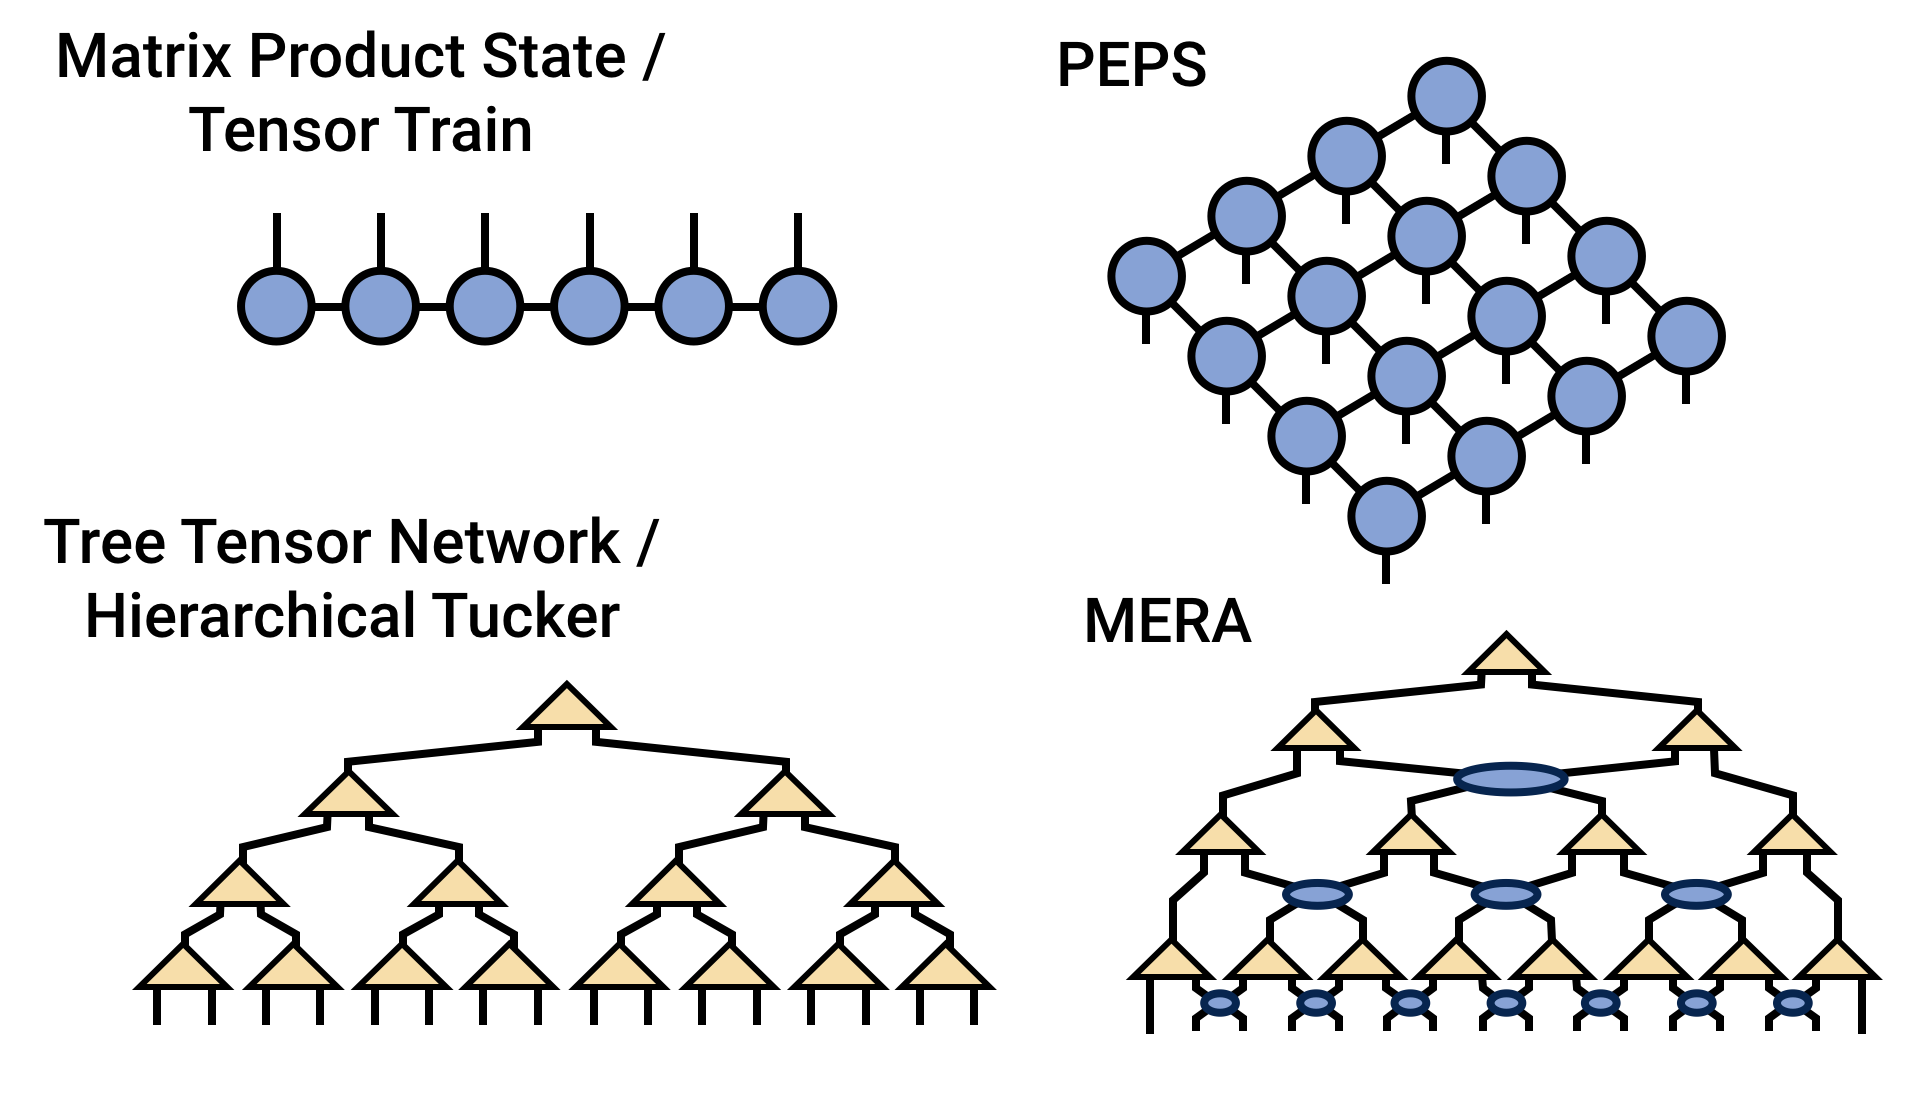
\includegraphics[width=0.45\textwidth]{img/tensor_networks.png}
    \caption{Tensor networks types}
    \label{fig:tensor_networks}
\end{figure}

TT represents the sequential decomposition of the high-dimensional $d$-way tensor $\mathcal{A}\in\mathbb{R}^{n_1\times n_2\times\dots\times n_d}$ with two $2$-way and $(d-2)$ $3$-way tensors in the following outer product:
\begin{equation}
    \label{eq:tt}
    \mathcal{A}=\mathcal{G}^{(1)}\circ\mathcal{G}^{(2)}\circ\dots\circ\mathcal{G}^{(d)}
\end{equation}
where $\mathcal{G}^{(k)}\in\mathbb{R}^{r_{k-1}\times n_k\times r_k}$ is the $k$-th core tensor, $r_k$ are the so-called {\itshape tensor-train (TT) ranks}. The MPS with low TT ranks has shown its efficiency for simulation of the quantum circuits with moderate entanglement generation capability \cite{Waintal2020}.

We demonstrate how the TT decomposition can improve the performance of the quantum state learning task. We implement the modified online learning algorithm  

\begin{figure}
    \centering
    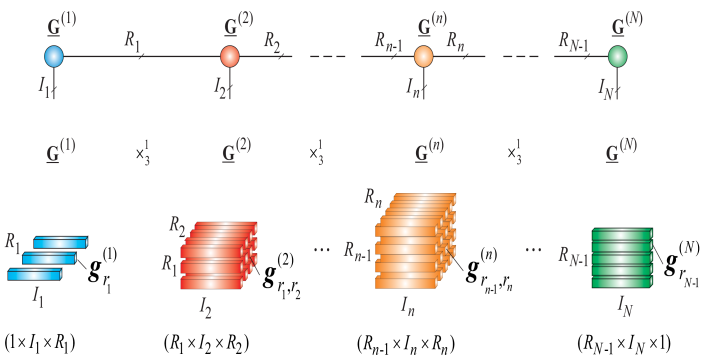
\includegraphics[width=0.45\textwidth]{img/tensor_train.png}
    \caption{Tensor Train (TT) \cite{tensorTrains, tensorTrainsOs}}
    \label{fig:tensor_trains}
\end{figure}

\section{\label{sec:algo}Learning algorithm}

In this work we use {\itshape locally purified tensor networks} in online quantum learning settings. Namely, our online-learning algorithm (Algorithm \ref{algo:our}) is explicit based on gradient descent of the hypothesis, approximated by {\itshape locally purified tensor networks}.

We use the Cholesky decomposition to enable positive semidefinite property of the hypothesis. The hypothesis $\omega$ is represented via the product of positive definite matrices $\omega = X^\dagger X$. The algorithm optimizes the matrix $X$ instead of direct optimization of the $\omega$. Since any $X^\dagger X$ is positive definite matrix and for any positive definite matrix Cholesky decomposition exists, we have an ensurance that fitting $X$ we will always provide positive definite hypothesis $\omega$. Trace normalization here can be performed in the same way like it was in MEG algorithm~\eqref{eq:meg}. The quantum state TT decomposition in conjunction with Cholesky decomposition is called {\itshape locally purified tensor networks} and was originally introduced in \cite{Werner_2016}.

\begin{algorithm}
\caption{Our algorithm\\}
\hspace*{\algorithmicindent} \textbf{Input}: $T,\eta$ \\
% \hspace*{\algorithmicindent} \textbf{Input}:\\
\begin{algorithmic}[1]
\State Set $X\coloneqq \text{TT}(2^{-n}\mathbb{I})$

\For{$t=1,\dots,T$}
    \State $\omega \coloneqq X^\dagger X$
    \State Consider the convex loss function $l_t : \mathbb{R} \rightarrow \mathbb{R}$ given by measurement $E_t : l_t(Tr(E_t\omega))$
    \State Update $X\coloneqq X-\eta\nabla_X l_t(Tr(E_t X^\dagger X))$
\EndFor

\end{algorithmic}
\label{algo:our}
\end{algorithm}

\section{\label{sec:sim}Simulations}

\section{\label{sec:exp}Experimental verification}
The performance of the algorithm \ref{algo:our} was certified using the experimental data collected using quantum states of light encoded in the transverse Hermite-Gaussian ($HG$) spatial modes. The $HG_{mn}(x,y)$ modes constitute discrete orthonormal basis in transverse spatial coordinates, where indices $m,n$ enumerate modes in $X$ and $Y$ axes respectively. Each mode is identified by the order $k = m+n$. The maximal order mode we prepare in the experiment depends on the dimensionality $D$ of the quantum system under study. Given the required dimension value $D$ the $k_{max}$ is the minimal integer number satisfying the inequality $(k_{max}+1)(k_{max}+2)/2 \geq D$. We have tested the algorithm \ref{algo:our} using the state dimensions $D =2,4,8,16,32$.

The experimental setup is illustrated in Fig. \ref{}. We use weak coherent states of light produced by the 808 nm laser diode. The spatial mode of the diode beam is filtered using the single-mode fiber (SMF-1). We employ the single spatial light modulator (SLM) to enable both state preparation and measurement in $HG_{mn}$ mode basis. The top half of the SLM reflective liquid crystal screen displays the hologram designed for preparation of the desired state and the bottom half in pair with the single-mode fiber (SMF-2) implements the projective measurements \cite{Bent2015, Palmieri2020}. The holograms on the SLM include blazed grating to induce beam mode amplitude modulation \cite{Bolduc2013} thus we use the pinhole to select only the first diffraction order. We note that optimal $HG$ mode preparation and measurement is achieved only after the Gouy phase of the beam is taken into account \cite{Struchalin2020}.

The dataset was generated by projecting the quantum state $\rho$ onto 5000 Haar-random sampled vectors $\left|\chi_{i}\right\rangle$. The full dataset was divided into two collections. The first one served as the training set for learning the hypothesis $\omega$. The elements of the second set were used to run the cross-validation procedure which proves the predictive strength of the $\omega$. The Fig. \ref{} summarizes the results of the experiment. 

\section{\label{sec:discuss}Discussion}

\section{\label{sec:acknowledge}Acknowledgements}

\bibliography{apssamp}% Produces the bibliography via BibTeX.

\end{document}
%
% ****** End of file apssamp.tex ******
